\section{System Design}

\subsection{Hardware Design}
The hardware design of the smart home system includes both the physical components and their connections. We utilized SolidWorks for designing the physical layout and circuits for our smart home.

\subsubsection{SolidWorks Design}
The design process for our smart home system began with creating detailed 3D models using SolidWorks software. We meticulously crafted each component, ensuring precise dimensions and proper fit for seamless integration into the final system.

\begin{figure}[htbp]
    \centering
    \begin{minipage}[t]{0.2\textwidth}
        \centering
        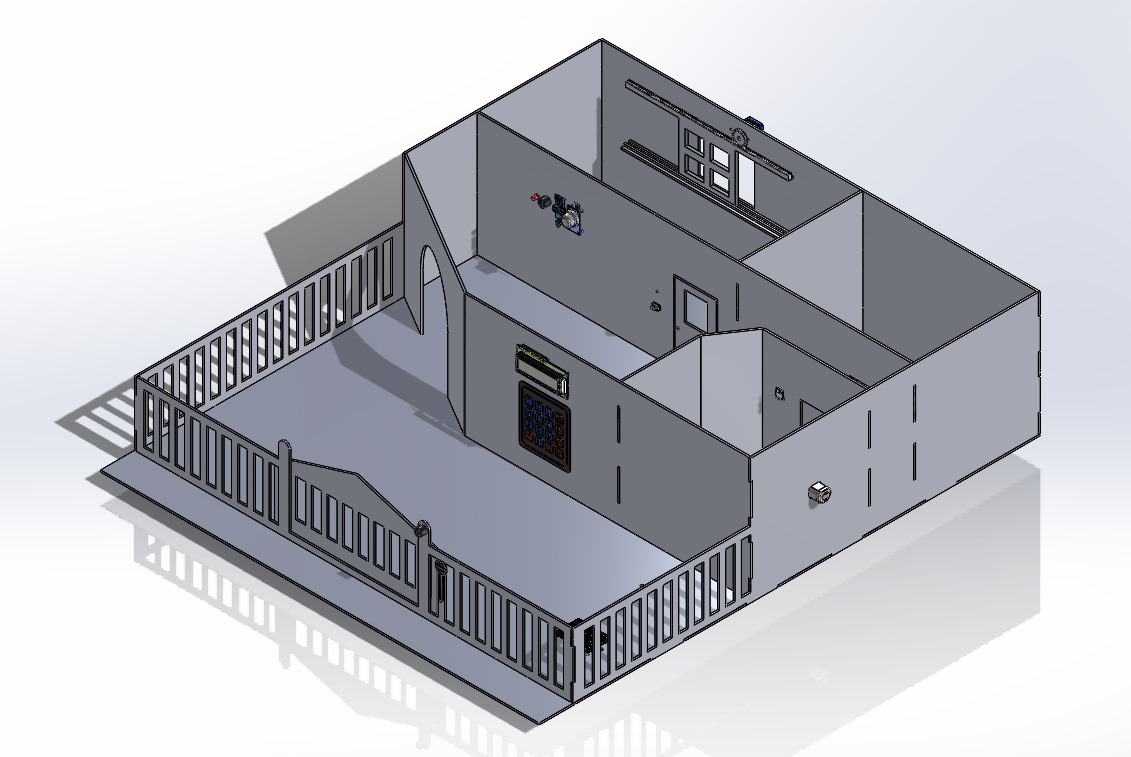
\includegraphics[width=\textwidth]{figs/Smart_Home1.jpg}
    \end{minipage}
    \hfill
    \begin{minipage}[t]{0.2\textwidth}
        \centering
        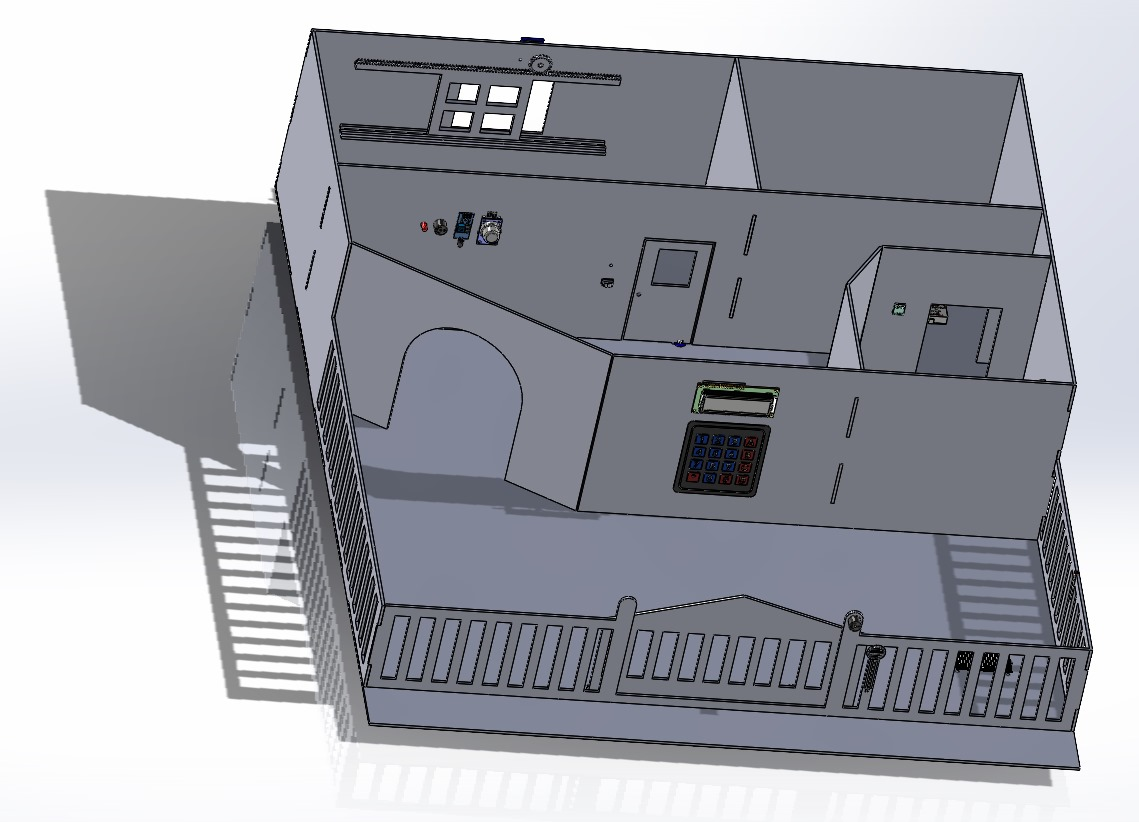
\includegraphics[width=\textwidth]{figs/Smart_Home2.jpg}
    \end{minipage}
    \hfill
    \begin{minipage}[t]{0.2\textwidth}
        \centering
        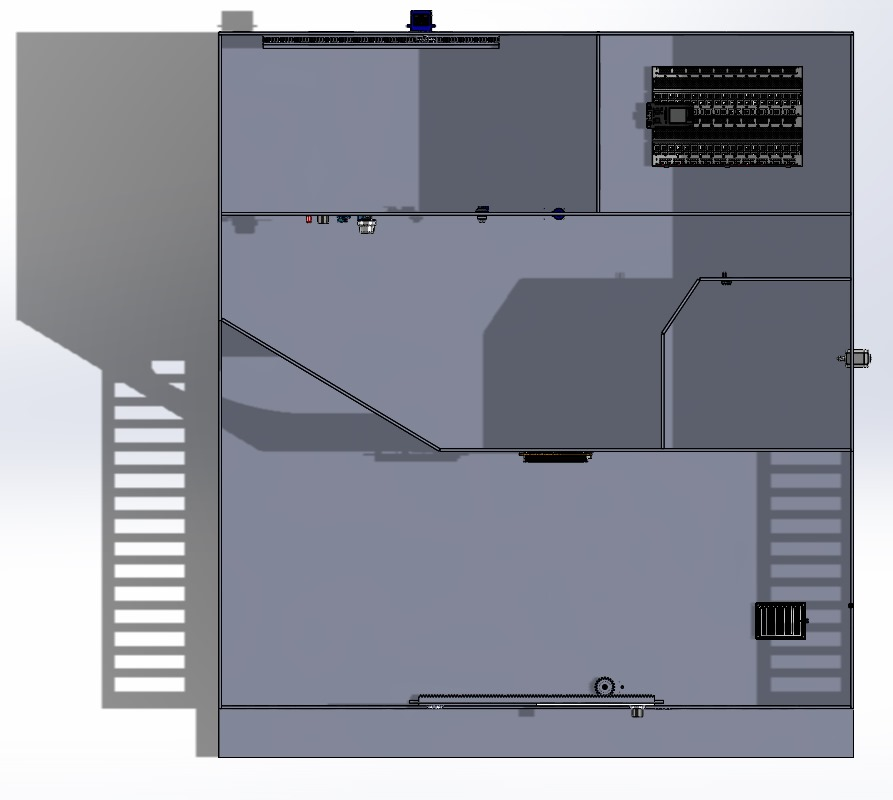
\includegraphics[width=\textwidth]{figs/Smart_Home3.jpg}
    \end{minipage}
    \hfill
    \begin{minipage}[t]{0.2\textwidth}
        \centering
        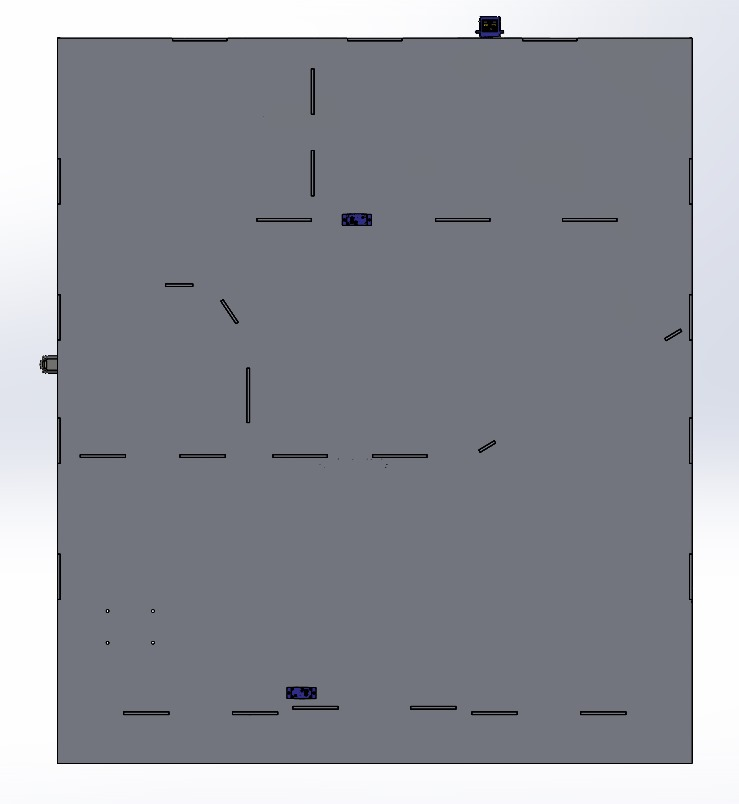
\includegraphics[width=\textwidth]{figs/Smart_Home4.jpg}
    \end{minipage}
\end{figure}

\begin{figure}[htbp]
    \centering
    \begin{minipage}[t]{0.2\textwidth}
        \centering
        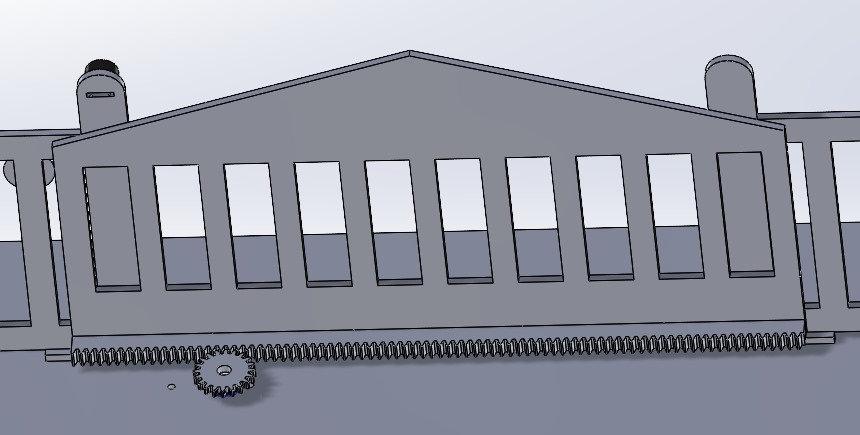
\includegraphics[width=\textwidth]{figs/Smart_Home5.jpg}
    \end{minipage}
    \hfill
    \begin{minipage}[t]{0.2\textwidth}
        \centering
        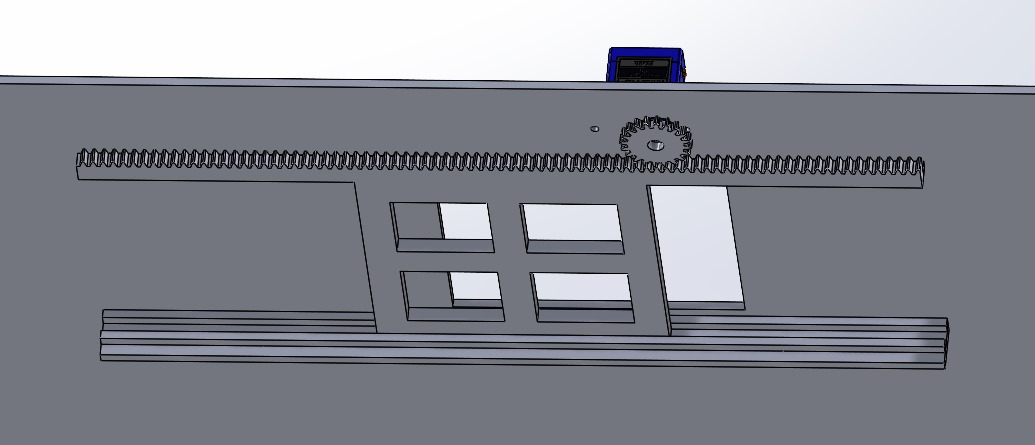
\includegraphics[width=\textwidth]{figs/Smart_Home6.jpg}
    \end{minipage}
    \hfill
    \begin{minipage}[t]{0.2\textwidth}
        \centering
        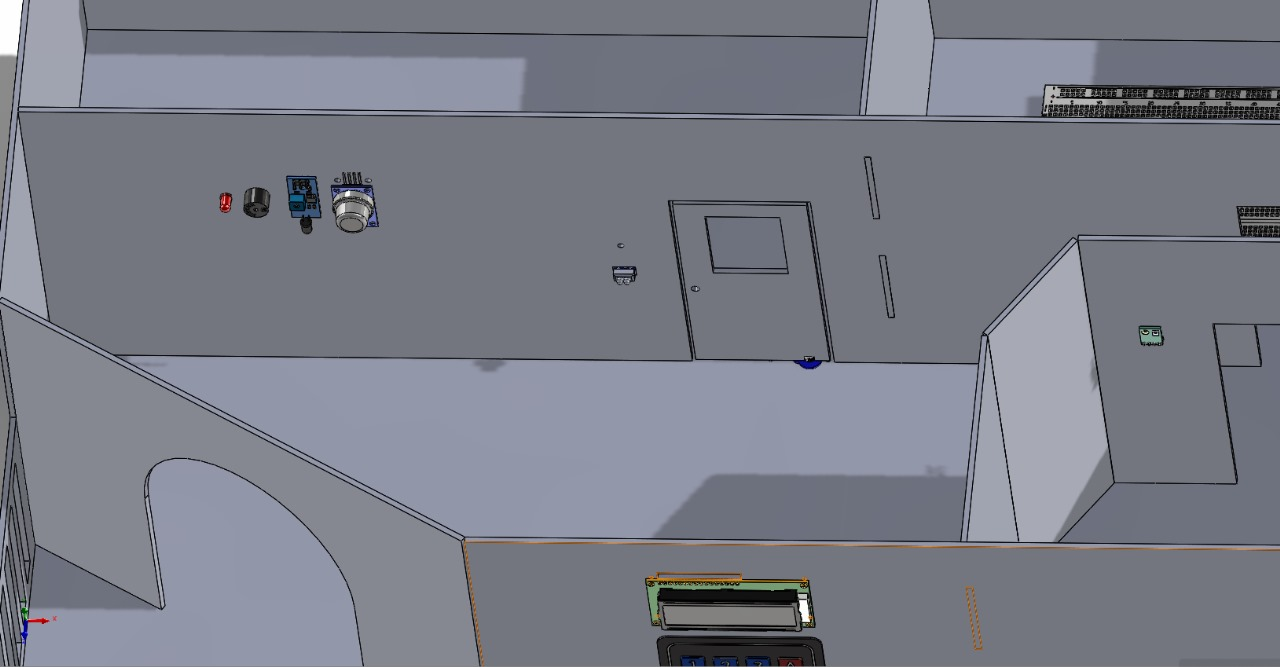
\includegraphics[width=\textwidth]{figs/Smart_Home7.jpg}
    \end{minipage}
    \hfill
    \begin{minipage}[t]{0.2\textwidth}
        \centering
        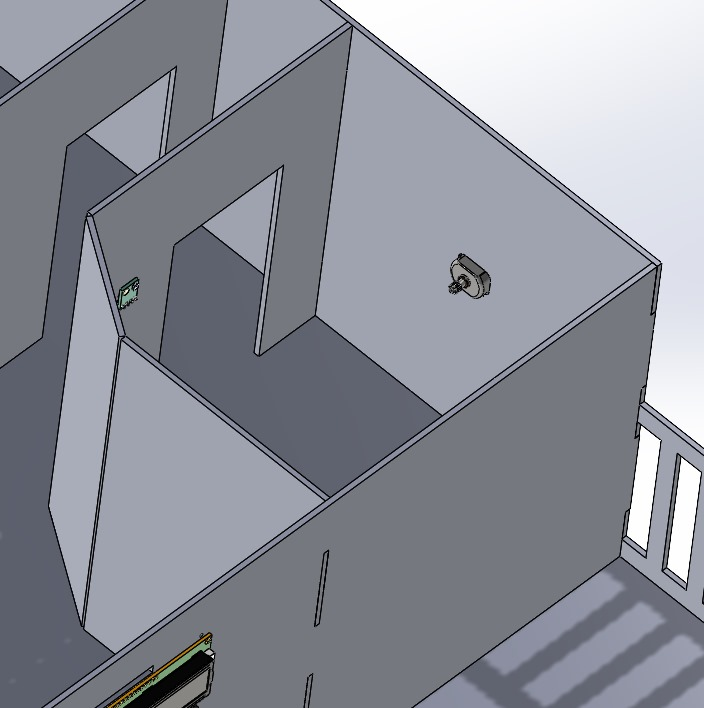
\includegraphics[width=\textwidth]{figs/Smart_Home8.jpg}
    \end{minipage}
\end{figure}



\subsubsection{Circuit Design}
The circuit design for our smart home system was meticulously planned to ensure reliable performance and efficient operation. We carefully selected components and designed circuit layouts to optimize functionality and minimize space requirements.

\begin{figure}[htbp]
    \centering
    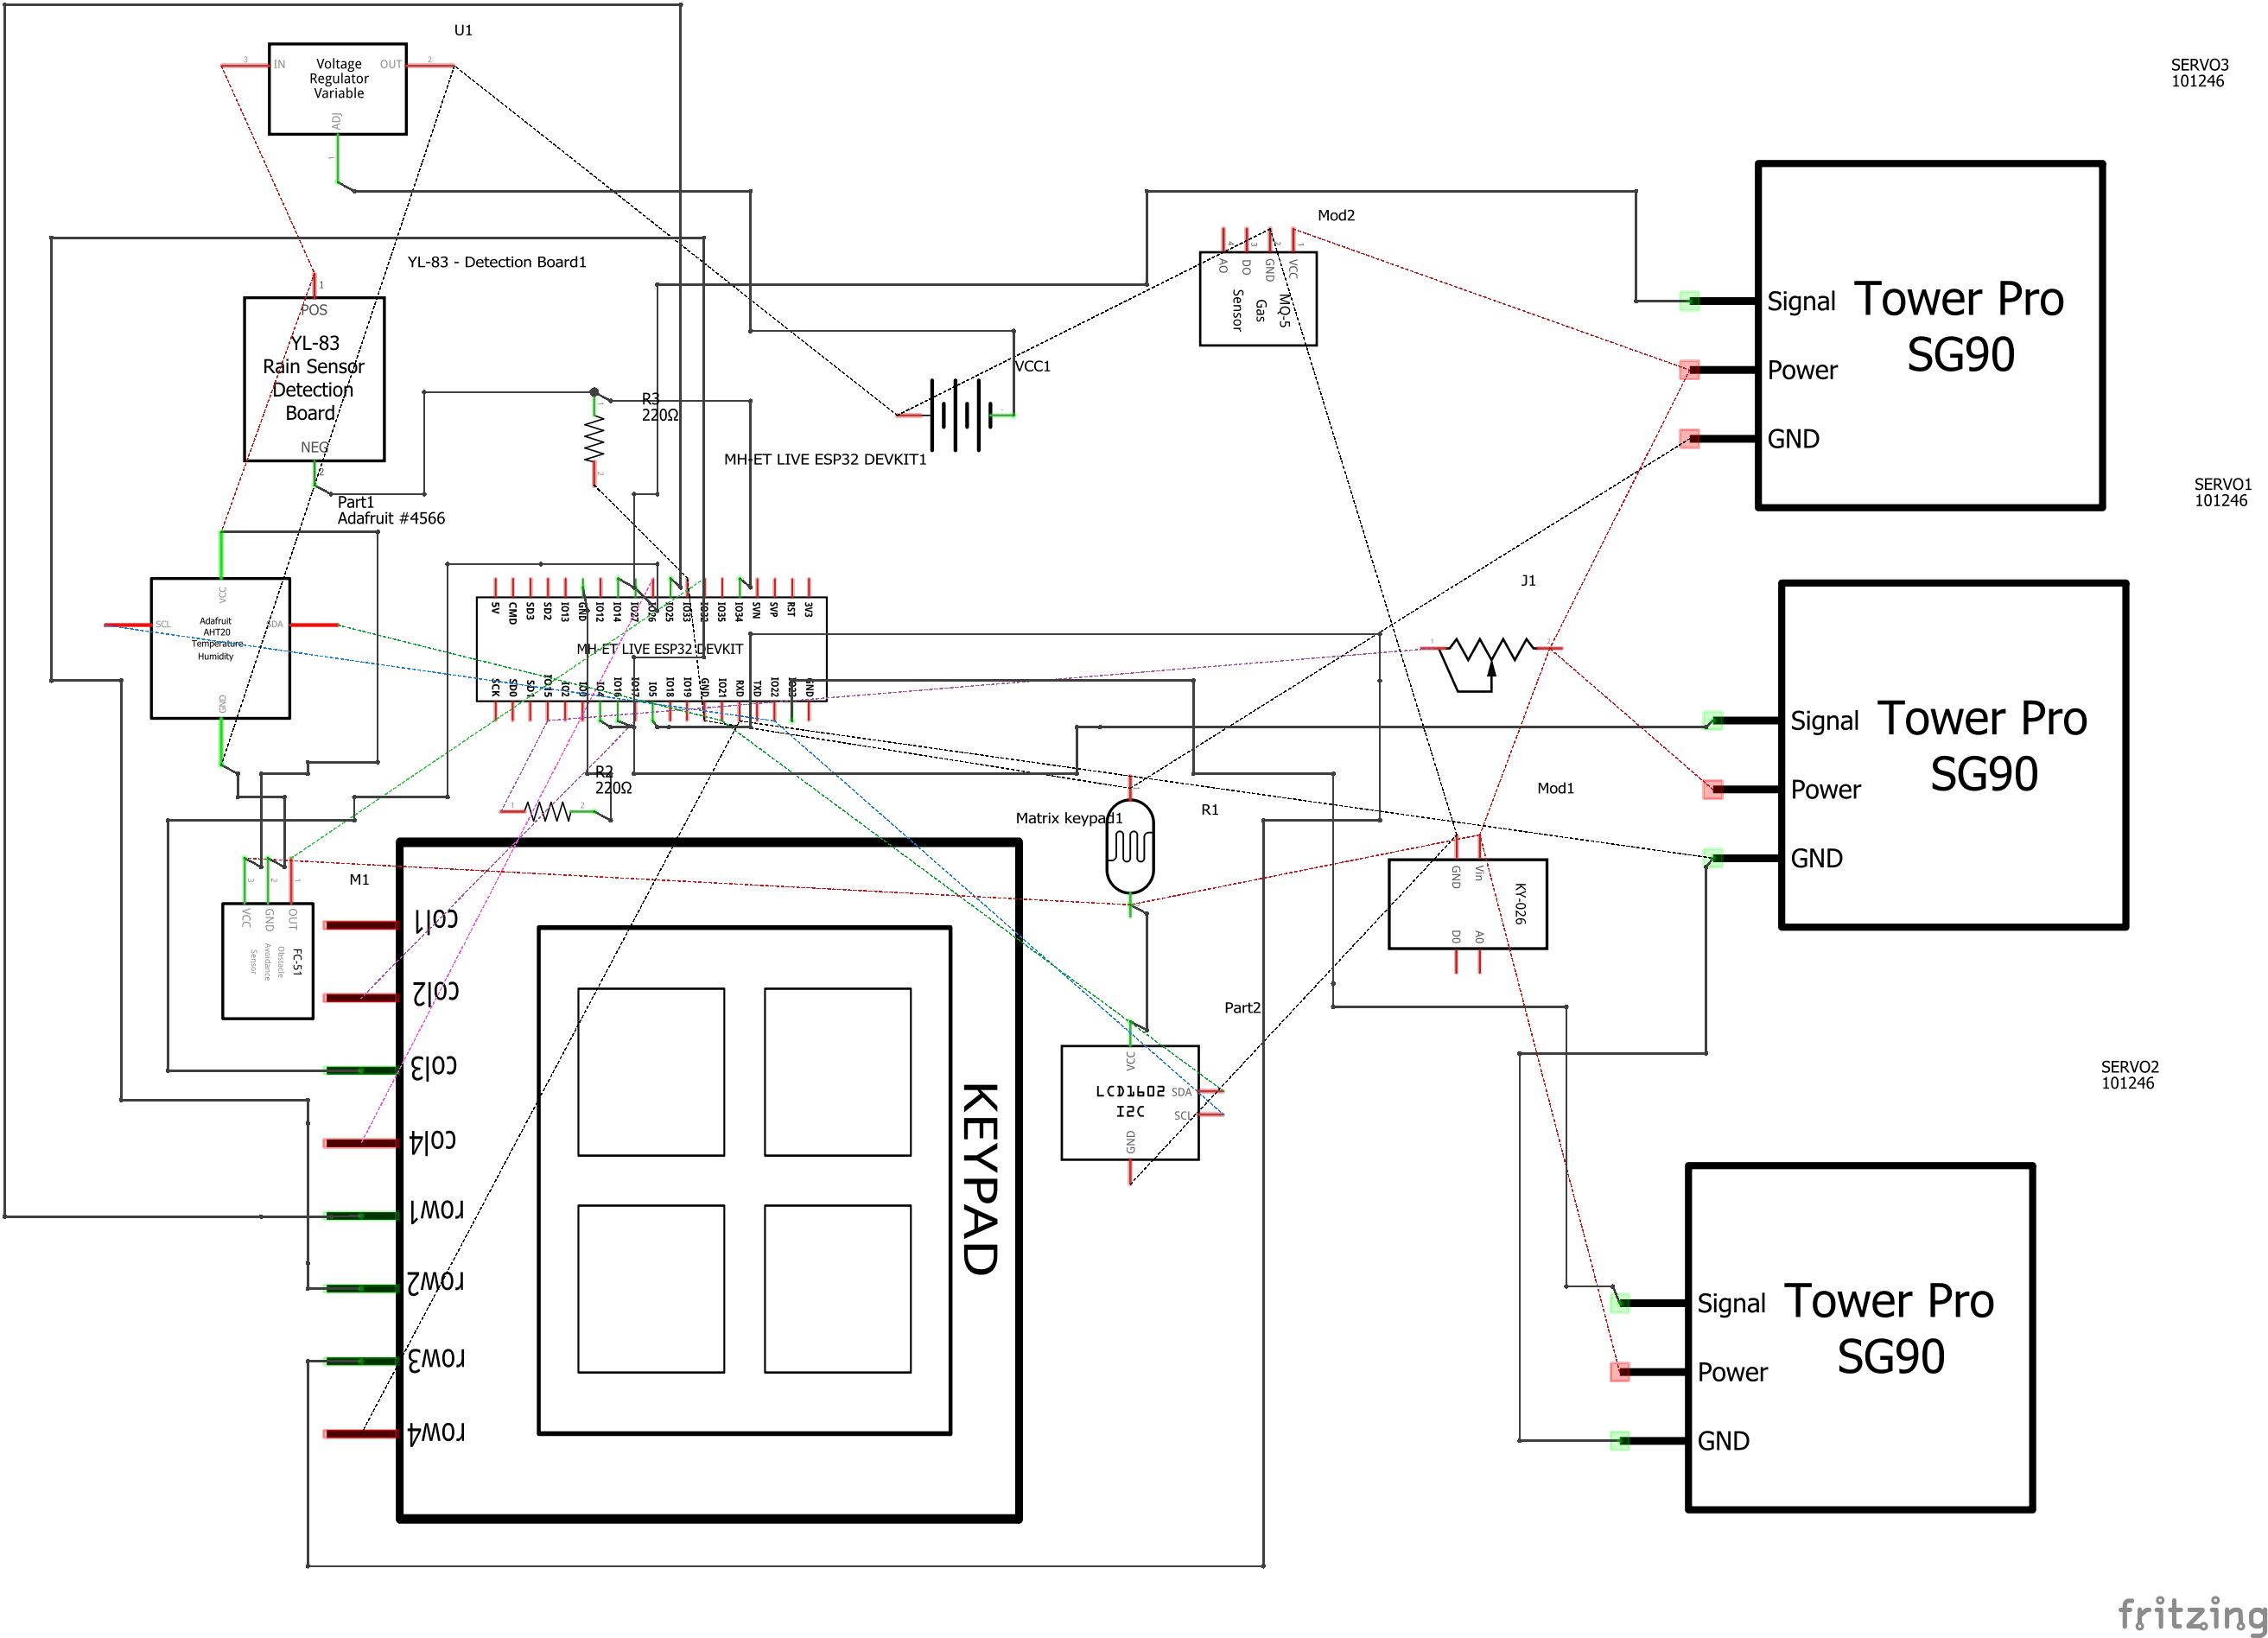
\includegraphics[width=0.8\textwidth]{figs/Smart_Home_Schema.png}
    \caption{Circuit Diagram}
    \label{fig:circuit_diagram}
\end{figure}

The circuit consists of various sensors, actuators, and the ESP32 microcontroller, all interconnected to enable seamless communication and control. Each component plays a crucial role in monitoring and managing different aspects of the smart home environment.

Detailed attention was given to wiring configurations and component placement to ensure efficient signal transmission and minimize interference. The circuit design underwent rigorous testing and refinement to achieve optimal performance and reliability in real-world conditions.


\subsection{Software System Design}
The software architecture of our smart home system plays a crucial role in ensuring seamless communication, efficient data processing, and robust control mechanisms. Here, we provide an overview of the key components, their roles, and design considerations in our software system.

\begin{itemize}
    \item \textbf{Firebase Integration}: Firebase Realtime Database serves as the backbone of our smart home system, facilitating real-time communication and data exchange between the ESP32 microcontroller, mobile application, and cloud server. Firebase provides a reliable and scalable platform for storing sensor data, user commands, and system configurations. The ESP32 microcontroller communicates with Firebase through secure HTTPS requests, enabling seamless synchronization of data and control commands.

    \item \textbf{WiFi Connectivity}: The ESP32 microcontroller relies on WiFi connectivity to establish communication with the Firebase server and receive commands from the mobile application. WiFi connectivity enables remote monitoring and control of the smart home systems, allowing users to access and manage their devices from anywhere with an internet connection. The ESP32 utilizes the WiFiClientSecure library to establish a secure connection with the Firebase server, ensuring data privacy and integrity.

    \item \textbf{Sensor Data Processing}: Sensor data collected from various devices, including temperature sensors, humidity sensors, rain sensors, flame sensors, and motion sensors, undergo real-time processing and analysis to detect environmental changes and trigger appropriate actions. The ESP32 microcontroller applies threshold-based algorithms and conditional logic to interpret sensor readings and make informed decisions. For example, it monitors temperature and humidity levels to adjust HVAC systems, detects smoke or flames to activate fire alarms, and senses motion to trigger security alerts.

    \item \textbf{Actuator Control}: Actuators such as servos, relays, and buzzers are controlled based on the commands received from the Firebase server or user inputs via the mobile application. The ESP32 microcontroller translates high-level commands into low-level control signals to actuate devices such as doors, windows, gates, fans, and alarms. For instance, it adjusts servo angles to open or close doors and windows, toggles relay states to control lighting and HVAC systems, and activates buzzers or sirens in response to security events.

    \item \textbf{Security Measures}: Robust security measures are integrated into the software system to protect against unauthorized access and potential threats. The ESP32 microcontroller implements secure authentication mechanisms, such as password authentication and keypad input validation, to verify user identity before granting access to critical functions and sensitive data. Additionally, it employs encryption protocols and secure communication channels to prevent eavesdropping and data tampering during transmission over WiFi networks.
\end{itemize}

The software system design is characterized by its modular architecture, which facilitates easy scalability, maintainability, and extensibility. Each component operates independently, yet collaboratively, to ensure the reliable and efficient operation of the smart home system. The use of well-defined interfaces and abstraction layers enables seamless integration of new sensors, actuators, and functionalities, making the smart home system adaptable to evolving requirements and emerging technologies.